% Options for packages loaded elsewhere
\PassOptionsToPackage{unicode}{hyperref}
\PassOptionsToPackage{hyphens}{url}
\PassOptionsToPackage{dvipsnames,svgnames,x11names}{xcolor}
%
\documentclass[
  letterpaper,
  DIV=11,
  numbers=noendperiod]{scrreprt}

\usepackage{amsmath,amssymb}
\usepackage{iftex}
\ifPDFTeX
  \usepackage[T1]{fontenc}
  \usepackage[utf8]{inputenc}
  \usepackage{textcomp} % provide euro and other symbols
\else % if luatex or xetex
  \usepackage{unicode-math}
  \defaultfontfeatures{Scale=MatchLowercase}
  \defaultfontfeatures[\rmfamily]{Ligatures=TeX,Scale=1}
\fi
\usepackage{lmodern}
\ifPDFTeX\else  
    % xetex/luatex font selection
\fi
% Use upquote if available, for straight quotes in verbatim environments
\IfFileExists{upquote.sty}{\usepackage{upquote}}{}
\IfFileExists{microtype.sty}{% use microtype if available
  \usepackage[]{microtype}
  \UseMicrotypeSet[protrusion]{basicmath} % disable protrusion for tt fonts
}{}
\makeatletter
\@ifundefined{KOMAClassName}{% if non-KOMA class
  \IfFileExists{parskip.sty}{%
    \usepackage{parskip}
  }{% else
    \setlength{\parindent}{0pt}
    \setlength{\parskip}{6pt plus 2pt minus 1pt}}
}{% if KOMA class
  \KOMAoptions{parskip=half}}
\makeatother
\usepackage{xcolor}
\setlength{\emergencystretch}{3em} % prevent overfull lines
\setcounter{secnumdepth}{5}
% Make \paragraph and \subparagraph free-standing
\makeatletter
\ifx\paragraph\undefined\else
  \let\oldparagraph\paragraph
  \renewcommand{\paragraph}{
    \@ifstar
      \xxxParagraphStar
      \xxxParagraphNoStar
  }
  \newcommand{\xxxParagraphStar}[1]{\oldparagraph*{#1}\mbox{}}
  \newcommand{\xxxParagraphNoStar}[1]{\oldparagraph{#1}\mbox{}}
\fi
\ifx\subparagraph\undefined\else
  \let\oldsubparagraph\subparagraph
  \renewcommand{\subparagraph}{
    \@ifstar
      \xxxSubParagraphStar
      \xxxSubParagraphNoStar
  }
  \newcommand{\xxxSubParagraphStar}[1]{\oldsubparagraph*{#1}\mbox{}}
  \newcommand{\xxxSubParagraphNoStar}[1]{\oldsubparagraph{#1}\mbox{}}
\fi
\makeatother

\usepackage{color}
\usepackage{fancyvrb}
\newcommand{\VerbBar}{|}
\newcommand{\VERB}{\Verb[commandchars=\\\{\}]}
\DefineVerbatimEnvironment{Highlighting}{Verbatim}{commandchars=\\\{\}}
% Add ',fontsize=\small' for more characters per line
\usepackage{framed}
\definecolor{shadecolor}{RGB}{241,243,245}
\newenvironment{Shaded}{\begin{snugshade}}{\end{snugshade}}
\newcommand{\AlertTok}[1]{\textcolor[rgb]{0.68,0.00,0.00}{#1}}
\newcommand{\AnnotationTok}[1]{\textcolor[rgb]{0.37,0.37,0.37}{#1}}
\newcommand{\AttributeTok}[1]{\textcolor[rgb]{0.40,0.45,0.13}{#1}}
\newcommand{\BaseNTok}[1]{\textcolor[rgb]{0.68,0.00,0.00}{#1}}
\newcommand{\BuiltInTok}[1]{\textcolor[rgb]{0.00,0.23,0.31}{#1}}
\newcommand{\CharTok}[1]{\textcolor[rgb]{0.13,0.47,0.30}{#1}}
\newcommand{\CommentTok}[1]{\textcolor[rgb]{0.37,0.37,0.37}{#1}}
\newcommand{\CommentVarTok}[1]{\textcolor[rgb]{0.37,0.37,0.37}{\textit{#1}}}
\newcommand{\ConstantTok}[1]{\textcolor[rgb]{0.56,0.35,0.01}{#1}}
\newcommand{\ControlFlowTok}[1]{\textcolor[rgb]{0.00,0.23,0.31}{\textbf{#1}}}
\newcommand{\DataTypeTok}[1]{\textcolor[rgb]{0.68,0.00,0.00}{#1}}
\newcommand{\DecValTok}[1]{\textcolor[rgb]{0.68,0.00,0.00}{#1}}
\newcommand{\DocumentationTok}[1]{\textcolor[rgb]{0.37,0.37,0.37}{\textit{#1}}}
\newcommand{\ErrorTok}[1]{\textcolor[rgb]{0.68,0.00,0.00}{#1}}
\newcommand{\ExtensionTok}[1]{\textcolor[rgb]{0.00,0.23,0.31}{#1}}
\newcommand{\FloatTok}[1]{\textcolor[rgb]{0.68,0.00,0.00}{#1}}
\newcommand{\FunctionTok}[1]{\textcolor[rgb]{0.28,0.35,0.67}{#1}}
\newcommand{\ImportTok}[1]{\textcolor[rgb]{0.00,0.46,0.62}{#1}}
\newcommand{\InformationTok}[1]{\textcolor[rgb]{0.37,0.37,0.37}{#1}}
\newcommand{\KeywordTok}[1]{\textcolor[rgb]{0.00,0.23,0.31}{\textbf{#1}}}
\newcommand{\NormalTok}[1]{\textcolor[rgb]{0.00,0.23,0.31}{#1}}
\newcommand{\OperatorTok}[1]{\textcolor[rgb]{0.37,0.37,0.37}{#1}}
\newcommand{\OtherTok}[1]{\textcolor[rgb]{0.00,0.23,0.31}{#1}}
\newcommand{\PreprocessorTok}[1]{\textcolor[rgb]{0.68,0.00,0.00}{#1}}
\newcommand{\RegionMarkerTok}[1]{\textcolor[rgb]{0.00,0.23,0.31}{#1}}
\newcommand{\SpecialCharTok}[1]{\textcolor[rgb]{0.37,0.37,0.37}{#1}}
\newcommand{\SpecialStringTok}[1]{\textcolor[rgb]{0.13,0.47,0.30}{#1}}
\newcommand{\StringTok}[1]{\textcolor[rgb]{0.13,0.47,0.30}{#1}}
\newcommand{\VariableTok}[1]{\textcolor[rgb]{0.07,0.07,0.07}{#1}}
\newcommand{\VerbatimStringTok}[1]{\textcolor[rgb]{0.13,0.47,0.30}{#1}}
\newcommand{\WarningTok}[1]{\textcolor[rgb]{0.37,0.37,0.37}{\textit{#1}}}

\providecommand{\tightlist}{%
  \setlength{\itemsep}{0pt}\setlength{\parskip}{0pt}}\usepackage{longtable,booktabs,array}
\usepackage{calc} % for calculating minipage widths
% Correct order of tables after \paragraph or \subparagraph
\usepackage{etoolbox}
\makeatletter
\patchcmd\longtable{\par}{\if@noskipsec\mbox{}\fi\par}{}{}
\makeatother
% Allow footnotes in longtable head/foot
\IfFileExists{footnotehyper.sty}{\usepackage{footnotehyper}}{\usepackage{footnote}}
\makesavenoteenv{longtable}
\usepackage{graphicx}
\makeatletter
\newsavebox\pandoc@box
\newcommand*\pandocbounded[1]{% scales image to fit in text height/width
  \sbox\pandoc@box{#1}%
  \Gscale@div\@tempa{\textheight}{\dimexpr\ht\pandoc@box+\dp\pandoc@box\relax}%
  \Gscale@div\@tempb{\linewidth}{\wd\pandoc@box}%
  \ifdim\@tempb\p@<\@tempa\p@\let\@tempa\@tempb\fi% select the smaller of both
  \ifdim\@tempa\p@<\p@\scalebox{\@tempa}{\usebox\pandoc@box}%
  \else\usebox{\pandoc@box}%
  \fi%
}
% Set default figure placement to htbp
\def\fps@figure{htbp}
\makeatother

\KOMAoption{captions}{tableheading}
\makeatletter
\@ifpackageloaded{tcolorbox}{}{\usepackage[skins,breakable]{tcolorbox}}
\@ifpackageloaded{fontawesome5}{}{\usepackage{fontawesome5}}
\definecolor{quarto-callout-color}{HTML}{909090}
\definecolor{quarto-callout-note-color}{HTML}{0758E5}
\definecolor{quarto-callout-important-color}{HTML}{CC1914}
\definecolor{quarto-callout-warning-color}{HTML}{EB9113}
\definecolor{quarto-callout-tip-color}{HTML}{00A047}
\definecolor{quarto-callout-caution-color}{HTML}{FC5300}
\definecolor{quarto-callout-color-frame}{HTML}{acacac}
\definecolor{quarto-callout-note-color-frame}{HTML}{4582ec}
\definecolor{quarto-callout-important-color-frame}{HTML}{d9534f}
\definecolor{quarto-callout-warning-color-frame}{HTML}{f0ad4e}
\definecolor{quarto-callout-tip-color-frame}{HTML}{02b875}
\definecolor{quarto-callout-caution-color-frame}{HTML}{fd7e14}
\makeatother
\makeatletter
\@ifpackageloaded{bookmark}{}{\usepackage{bookmark}}
\makeatother
\makeatletter
\@ifpackageloaded{caption}{}{\usepackage{caption}}
\AtBeginDocument{%
\ifdefined\contentsname
  \renewcommand*\contentsname{Table of contents}
\else
  \newcommand\contentsname{Table of contents}
\fi
\ifdefined\listfigurename
  \renewcommand*\listfigurename{List of Figures}
\else
  \newcommand\listfigurename{List of Figures}
\fi
\ifdefined\listtablename
  \renewcommand*\listtablename{List of Tables}
\else
  \newcommand\listtablename{List of Tables}
\fi
\ifdefined\figurename
  \renewcommand*\figurename{Figure}
\else
  \newcommand\figurename{Figure}
\fi
\ifdefined\tablename
  \renewcommand*\tablename{Table}
\else
  \newcommand\tablename{Table}
\fi
}
\@ifpackageloaded{float}{}{\usepackage{float}}
\floatstyle{ruled}
\@ifundefined{c@chapter}{\newfloat{codelisting}{h}{lop}}{\newfloat{codelisting}{h}{lop}[chapter]}
\floatname{codelisting}{Listing}
\newcommand*\listoflistings{\listof{codelisting}{List of Listings}}
\makeatother
\makeatletter
\makeatother
\makeatletter
\@ifpackageloaded{caption}{}{\usepackage{caption}}
\@ifpackageloaded{subcaption}{}{\usepackage{subcaption}}
\makeatother

\usepackage{bookmark}

\IfFileExists{xurl.sty}{\usepackage{xurl}}{} % add URL line breaks if available
\urlstyle{same} % disable monospaced font for URLs
\hypersetup{
  pdftitle={SpatialData.book},
  colorlinks=true,
  linkcolor={blue},
  filecolor={Maroon},
  citecolor={Blue},
  urlcolor={Blue},
  pdfcreator={LaTeX via pandoc}}


\title{SpatialData.book}
\author{}
\date{}

\begin{document}
\maketitle

\renewcommand*\contentsname{Table of contents}
{
\hypersetup{linkcolor=}
\setcounter{tocdepth}{2}
\tableofcontents
}

\bookmarksetup{startatroot}

\chapter*{Warning in packageDescription(``SpatialData.book''): no
package}\label{warning-in-packagedescriptionspatialdata.book-no-package}
\addcontentsline{toc}{chapter}{Warning in
packageDescription(``SpatialData.book''): no package}

\markboth{Warning in packageDescription(``SpatialData.book''): no
package}{Warning in packageDescription(``SpatialData.book''): no
package}

\begin{verbatim}
##  'SpatialData.book' was found
\end{verbatim}

Local preview

\bookmarksetup{startatroot}

\chapter*{Docker image}\label{docker-image}
\addcontentsline{toc}{chapter}{Docker image}

\markboth{Docker image}{Docker image}

A \texttt{Docker} image built from this repository is available here:

👉
\href{https://ghcr.io/HelenaLC/spatialdata.book}{ghcr.io/HelenaLC/spatialdata.book}
🐳

\begin{tcolorbox}[enhanced jigsaw, opacityback=0, toprule=.15mm, bottomtitle=1mm, rightrule=.15mm, breakable, bottomrule=.15mm, colframe=quarto-callout-tip-color-frame, colback=white, coltitle=black, left=2mm, titlerule=0mm, title=\textcolor{quarto-callout-tip-color}{\faLightbulb}\hspace{0.5em}{Get started now 🎉}, toptitle=1mm, arc=.35mm, colbacktitle=quarto-callout-tip-color!10!white, leftrule=.75mm, opacitybacktitle=0.6]

You can get access to all the packages used in this book in \textless{}
1 minute, using this command in a terminal:

\begin{codelisting}[H]

\caption{\texttt{bash}}

\begin{Shaded}
\begin{Highlighting}[]
\ExtensionTok{docker}\NormalTok{ run }\AttributeTok{{-}it}\NormalTok{ ghcr.io/HelenaLC/spatialdata.book:devel R}
\end{Highlighting}
\end{Shaded}

\end{codelisting}

\end{tcolorbox}

\bookmarksetup{startatroot}

\chapter*{RStudio Server}\label{rstudio-server}
\addcontentsline{toc}{chapter}{RStudio Server}

\markboth{RStudio Server}{RStudio Server}

An RStudio Server instance can be initiated from the \texttt{Docker}
image as follows:

\begin{codelisting}

\caption{\texttt{bash}}

\begin{Shaded}
\begin{Highlighting}[]
\ExtensionTok{docker}\NormalTok{ run }\DataTypeTok{\textbackslash{}}
    \AttributeTok{{-}{-}volume} \OperatorTok{\textless{}}\NormalTok{local\_folder}\OperatorTok{\textgreater{}}\NormalTok{:}\OperatorTok{\textless{}}\NormalTok{destination\_folder}\OperatorTok{\textgreater{}} \DataTypeTok{\textbackslash{}}
    \AttributeTok{{-}e}\NormalTok{ PASSWORD=OHCA }\DataTypeTok{\textbackslash{}}
    \AttributeTok{{-}p}\NormalTok{ 8787:8787 }\DataTypeTok{\textbackslash{}}
\NormalTok{    ghcr.io/HelenaLC/spatialdata.book:devel}
\end{Highlighting}
\end{Shaded}

\end{codelisting}

The initiated RStudio Server instance will be available at
\url{https://localhost:8787}.

\begin{tcolorbox}[enhanced jigsaw, opacityback=0, toprule=.15mm, bottomtitle=1mm, rightrule=.15mm, breakable, bottomrule=.15mm, colframe=quarto-callout-note-color-frame, colback=white, coltitle=black, left=2mm, titlerule=0mm, title=\textcolor{quarto-callout-note-color}{\faInfo}\hspace{0.5em}{Session info}, toptitle=1mm, arc=.35mm, colbacktitle=quarto-callout-note-color!10!white, leftrule=.75mm, opacitybacktitle=0.6]

\begin{Shaded}
\begin{Highlighting}[]
\FunctionTok{sessionInfo}\NormalTok{()}
\DocumentationTok{\#\#  R version 4.4.1 Patched (2024{-}07{-}08 r86893)}
\DocumentationTok{\#\#  Platform: aarch64{-}apple{-}darwin20}
\DocumentationTok{\#\#  Running under: macOS Sonoma 14.2.1}
\DocumentationTok{\#\#  }
\DocumentationTok{\#\#  Matrix products: default}
\DocumentationTok{\#\#  BLAS:   /Library/Frameworks/R.framework/Versions/4.4{-}arm64/Resources/lib/libRblas.0.dylib }
\DocumentationTok{\#\#  LAPACK: /Library/Frameworks/R.framework/Versions/4.4{-}arm64/Resources/lib/libRlapack.dylib;  LAPACK version 3.12.0}
\DocumentationTok{\#\#  }
\DocumentationTok{\#\#  locale:}
\DocumentationTok{\#\#  [1] en\_US.UTF{-}8/en\_US.UTF{-}8/en\_US.UTF{-}8/C/en\_US.UTF{-}8/en\_US.UTF{-}8}
\DocumentationTok{\#\#  }
\DocumentationTok{\#\#  time zone: Europe/Berlin}
\DocumentationTok{\#\#  tzcode source: internal}
\DocumentationTok{\#\#  }
\DocumentationTok{\#\#  attached base packages:}
\DocumentationTok{\#\#  [1] stats     graphics  grDevices utils     datasets  methods   base     }
\DocumentationTok{\#\#  }
\DocumentationTok{\#\#  loaded via a namespace (and not attached):}
\DocumentationTok{\#\#   [1] compiler\_4.4.1    fastmap\_1.2.0     cli\_3.6.3         tools\_4.4.1      }
\DocumentationTok{\#\#   [5] htmltools\_0.5.8.1 rstudioapi\_0.17.1 yaml\_2.3.10       rmarkdown\_2.29   }
\DocumentationTok{\#\#   [9] knitr\_1.49        jsonlite\_1.8.9    xfun\_0.49         digest\_0.6.37    }
\DocumentationTok{\#\#  [13] rlang\_1.1.4       evaluate\_1.0.1}
\end{Highlighting}
\end{Shaded}

\end{tcolorbox}

\bookmarksetup{startatroot}

\chapter{Introduction}\label{introduction}

@Marconato2024

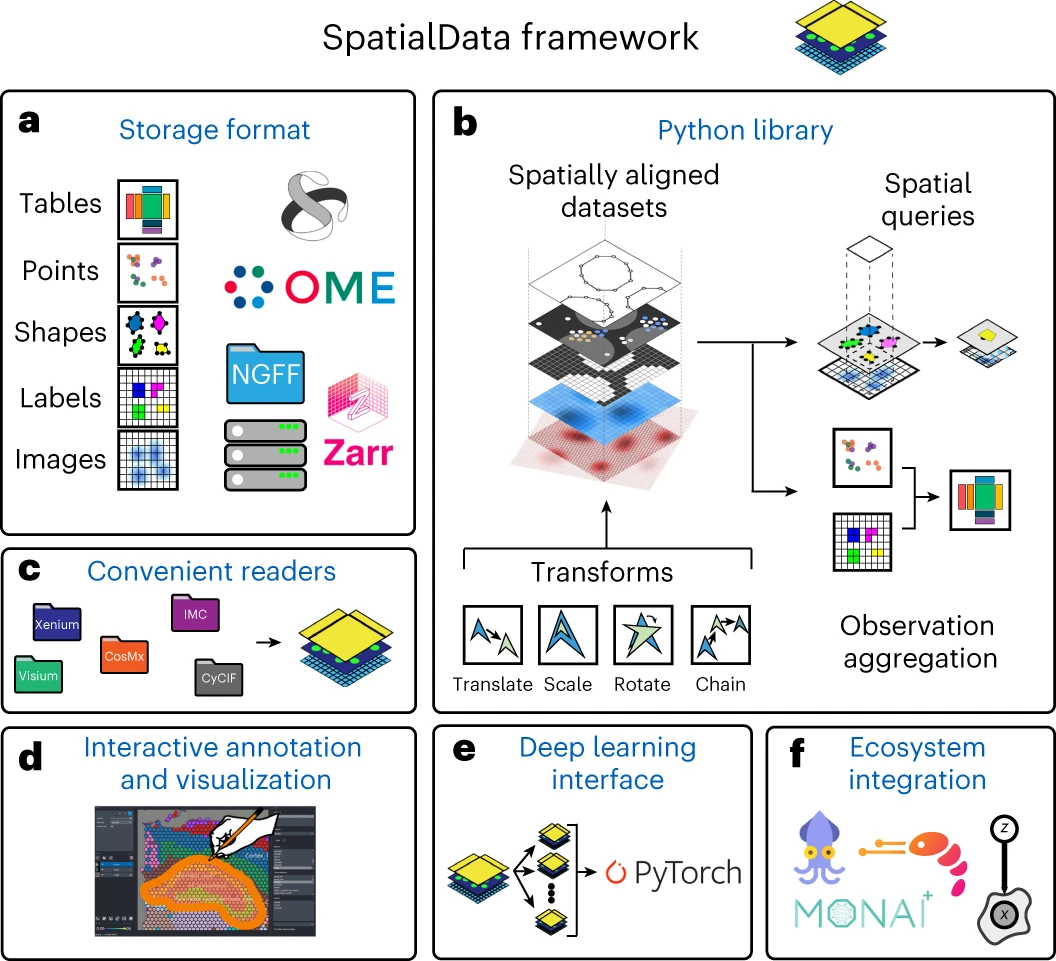
\includegraphics[width=0.5\linewidth,height=\textheight,keepaspectratio]{pages/images/SpatialData.png}

\begin{itemize}
\tightlist
\item
  \texttt{SpatialData}: S4 class, readers (and, not yet, writers)
\item
  \texttt{SpatialData.plot}: element-wise and layered visualization
\item
  \texttt{SpatialData.data}: example datasets made available\\
  through Bioc's OSN bucket (and
  \texttt{r\ BiocStyle::Biocpkg("BiocFileCache")} support)
\end{itemize}

\bookmarksetup{startatroot}

\chapter{Datasets}\label{datasets}

Datasets from
\href{https://spatialdata.scverse.org/en/latest/tutorials/notebooks/datasets/README.html}{spatialdata.scverse.org}
have been deposited in Bioconductor's OSN bucket, and can be loaded into
R using \texttt{SpatialData.data}, with support for caching using
\texttt{BiocFileCache}.

\begin{Shaded}
\begin{Highlighting}[]
\FunctionTok{library}\NormalTok{(SpatialData)}
\FunctionTok{library}\NormalTok{(SpatialData.data)}
\end{Highlighting}
\end{Shaded}

We can get a list of available datasets via:

\begin{Shaded}
\begin{Highlighting}[]
\FunctionTok{available\_spd\_zarr\_zips}\NormalTok{()}
\DocumentationTok{\#\#  [1] "mcmicro\_io.zip"                         }
\DocumentationTok{\#\#  [2] "merfish.zarr.zip"                       }
\DocumentationTok{\#\#  [3] "mibitof.zip"                            }
\DocumentationTok{\#\#  [4] "steinbock\_io.zip"                       }
\DocumentationTok{\#\#  [5] "visium\_associated\_xenium\_io\_aligned.zip"}
\DocumentationTok{\#\#  [6] "visium\_hd\_3.0.0\_io.zip"                 }
\DocumentationTok{\#\#  [7] "xenium\_rep1\_io\_aligned.zip"             }
\DocumentationTok{\#\#  [8] "xenium\_rep2\_io\_aligned.zip"}
\end{Highlighting}
\end{Shaded}

Any of the above can be retrieved using \texttt{unzip\_spd\_demo()}, and
read into a R using \texttt{readSpatialData()}; e.g.:

\begin{Shaded}
\begin{Highlighting}[]
\FunctionTok{dir.create}\NormalTok{(td }\OtherTok{\textless{}{-}} \FunctionTok{tempfile}\NormalTok{())}
\NormalTok{zs }\OtherTok{\textless{}{-}} \FunctionTok{unzip\_spd\_demo}\NormalTok{(}
    \AttributeTok{zipname=}\StringTok{"mibitof"}\NormalTok{, }
    \AttributeTok{source=}\StringTok{"biocOSN"}\NormalTok{,}
    \AttributeTok{destination=}\NormalTok{td)}
\NormalTok{(sd }\OtherTok{\textless{}{-}} \FunctionTok{readSpatialData}\NormalTok{(zs))}
\DocumentationTok{\#\#  class: SpatialData}
\DocumentationTok{\#\#  {-} images(3):}
\DocumentationTok{\#\#    {-} point16\_image (3,1024,1024)}
\DocumentationTok{\#\#    {-} point23\_image (3,1024,1024)}
\DocumentationTok{\#\#    {-} point8\_image (3,1024,1024)}
\DocumentationTok{\#\#  {-} labels(3):}
\DocumentationTok{\#\#    {-} point16\_labels (1024,1024)}
\DocumentationTok{\#\#    {-} point23\_labels (1024,1024)}
\DocumentationTok{\#\#    {-} point8\_labels (1024,1024)}
\DocumentationTok{\#\#  {-} points(0):}
\DocumentationTok{\#\#  {-} shapes(0):}
\DocumentationTok{\#\#  {-} tables(1):}
\DocumentationTok{\#\#    {-} table (36,3309)}
\DocumentationTok{\#\#  coordinate systems:}
\DocumentationTok{\#\#  {-} point16(2): point16\_image point16\_labels}
\DocumentationTok{\#\#  {-} point23(2): point23\_image point23\_labels}
\DocumentationTok{\#\#  {-} point8(2): point8\_image point8\_labels}
\end{Highlighting}
\end{Shaded}





\end{document}
